\documentclass{supervision}
\usepackage{course}

\Supervision{2}
\begin{document}
  \begin{questions}
    \section*{5 Constraint Satisfaction Problems}
    \question Consider the following constraint satisfaction problem:

      \begin{center}
        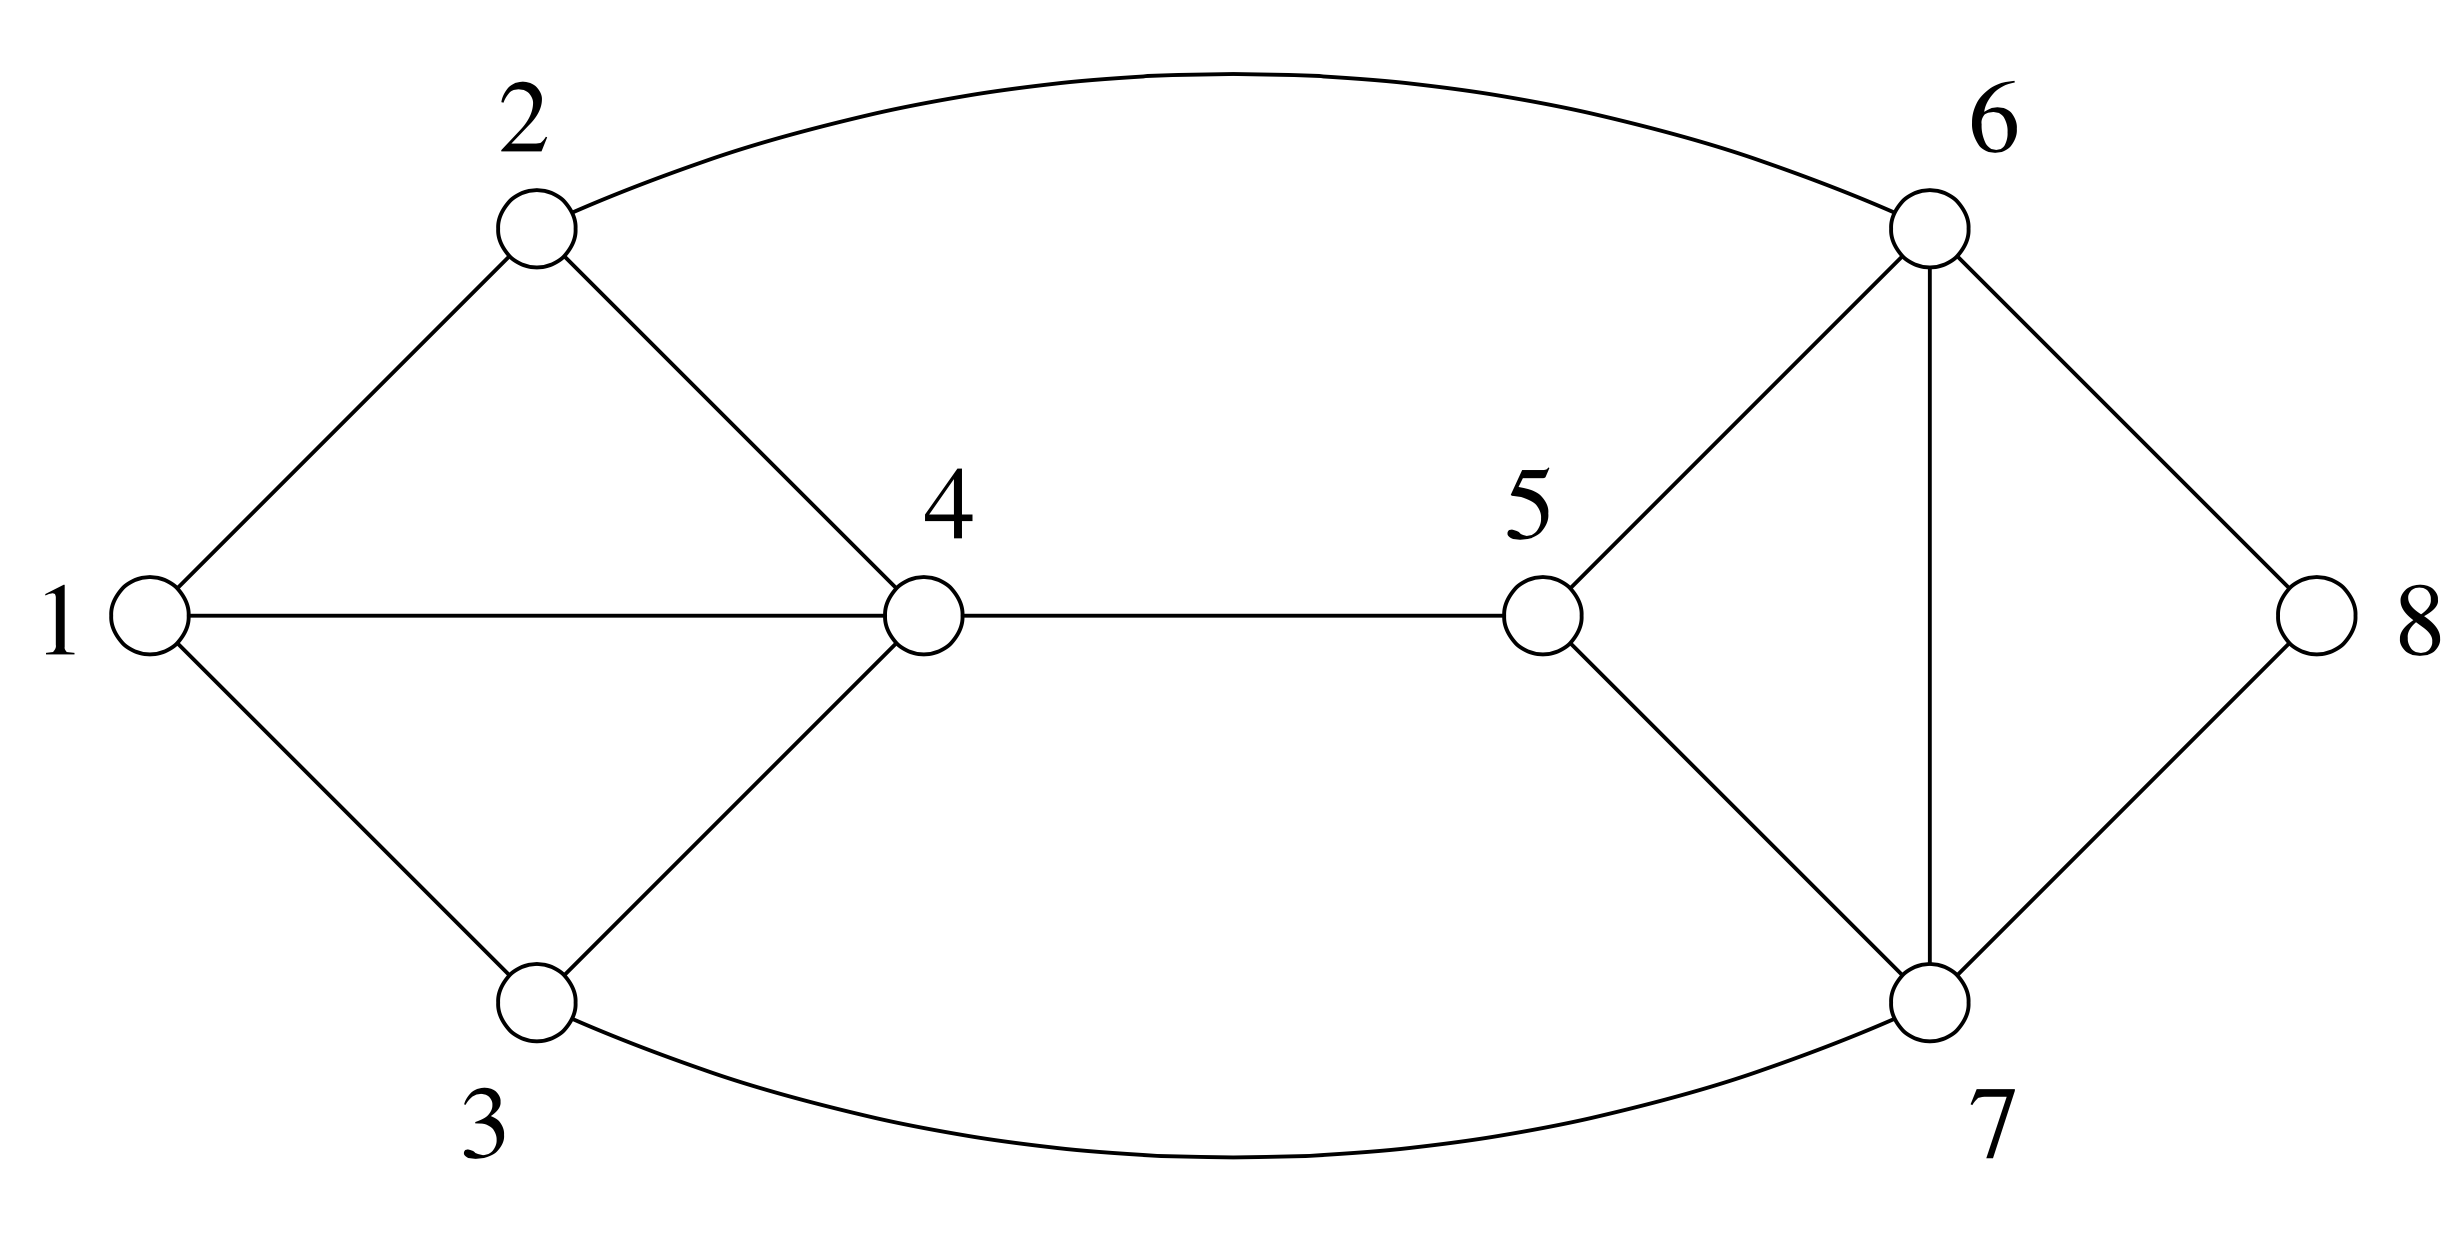
\includegraphics[width=0.7\textwidth]{2-graph}
      \end{center}

      We want to colour the nodes using the colours red (R), cyan (C) and black
      (B) in such a way that connected nodes have different colours.

      \begin{itemize}
        \item Assume we attempt the assignments $1 = R$, $4 = C$, $5 = R$, $8 =
          C$, $6 = B$. Explain how forward checking operates in this example,
          and how it detects the need to backtrack.

        \item Will the AC-3 algorithm detect a problem earlier in this case?
          Explain the operation of the algorithm in this example.

        \item Implement the AC-3 algorithm and use it to verify your answer to
          the preceding problem.
      \end{itemize}

    \section*{6 Knowledge representation and reasoning}
    \SetQuestionNumber{1}
    \question There have in fact been two queries suggested in the notes for
      obtaining a sequence of actions. The details for

      \begin{equation*}
        \exists a \exists s. {sequence}(a, s_0, s) \land {goal}(s)
      \end{equation*}

      were given on the last slide, but earlier in the notes the format

      \begin{equation*}
        \exists {actionList}.{Goal}(\ldots {actionList} \ldots)
      \end{equation*}

      was suggested. Explain how this alternative form of query might be made to
      work.

    \question Making correct use of the situation calculus, write the sentences
      in FOL required to implement the Shoot action in Wumpus World.

  \end{questions}
\end{document}
